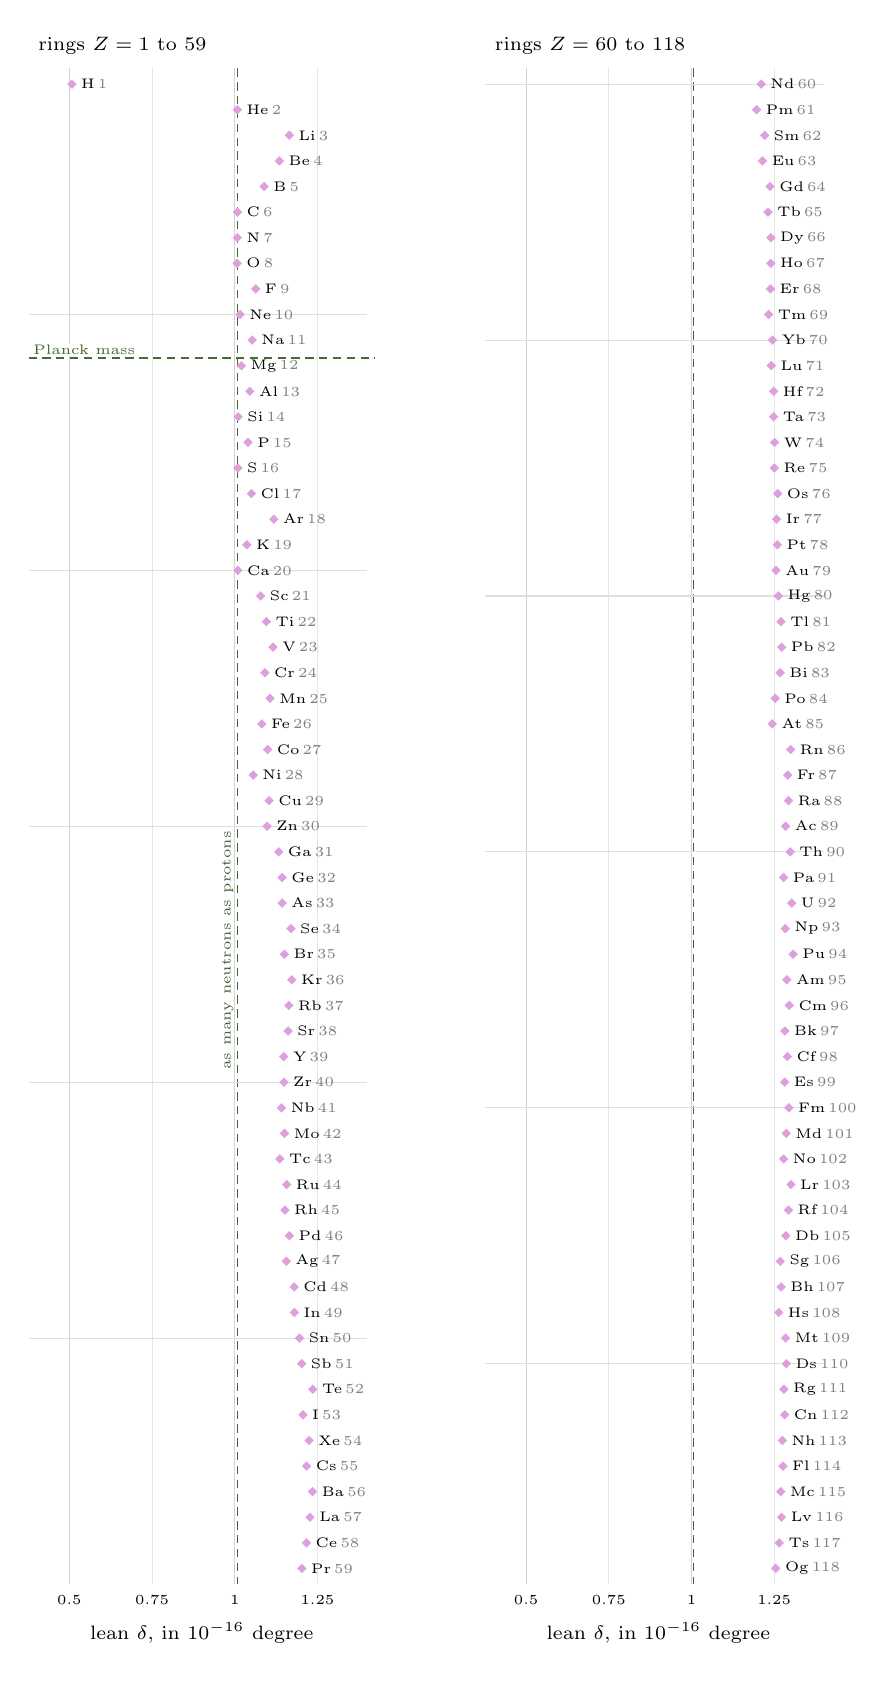
\begin{tikzpicture}[x=1mm, y=1mm, every node/.style={font=\tiny}]
\draw[gray!35] (4.2,2) -- (4.2,-190.5);
\node[anchor=north] at (4.2,-190.7) {0.5};
\draw[gray!20] (14.7,2) -- (14.7,-190.5);
\node[anchor=north] at (14.7,-190.7) {0.75};
\draw[gray!35] (25.2,2) -- (25.2,-190.5);
\node[anchor=north] at (25.2,-190.7) {1};
\draw[gray!20] (35.7,2) -- (35.7,-190.5);
\node[anchor=north] at (35.7,-190.7) {1.25};
\draw[OliveGreen!70!black, densely dashed] (25.51,2) -- (25.51,-190.5);
\node[anchor=north, align=center, font=\scriptsize] at (21,-194.1) {lean $\delta$, in $10^{-16}$ degree};
\draw[gray!25] (-1,-29.25) -- (42,-29.25);
\draw[gray!25] (-1,-61.75) -- (42,-61.75);
\draw[gray!25] (-1,-94.25) -- (42,-94.25);
\draw[gray!25] (-1,-126.75) -- (42,-126.75);
\draw[gray!25] (-1,-159.25) -- (42,-159.25);
\fill[Plum] (4.51,-0.6) -- ++(0.6,0.6) -- ++(-0.6,0.6) -- ++(-0.6,-0.6) -- cycle;
\node[anchor=west, inner sep=0.3pt] at (5.51,0) {H\,\textcolor{gray}{1}};
\fill[Plum] (25.53,-3.85) -- ++(0.6,0.6) -- ++(-0.6,0.6) -- ++(-0.6,-0.6) -- cycle;
\node[anchor=west, inner sep=0.3pt] at (26.53,-3.25) {He\,\textcolor{gray}{2}};
\fill[Plum] (32.13,-7.1) -- ++(0.6,0.6) -- ++(-0.6,0.6) -- ++(-0.6,-0.6) -- cycle;
\node[anchor=west, inner sep=0.3pt] at (33.13,-6.5) {Li\,\textcolor{gray}{3}};
\fill[Plum] (30.86,-10.35) -- ++(0.6,0.6) -- ++(-0.6,0.6) -- ++(-0.6,-0.6) -- cycle;
\node[anchor=west, inner sep=0.3pt] at (31.86,-9.75) {Be\,\textcolor{gray}{4}};
\fill[Plum] (28.93,-13.6) -- ++(0.6,0.6) -- ++(-0.6,0.6) -- ++(-0.6,-0.6) -- cycle;
\node[anchor=west, inner sep=0.3pt] at (29.93,-13) {B\,\textcolor{gray}{5}};
\fill[Plum] (25.54,-16.85) -- ++(0.6,0.6) -- ++(-0.6,0.6) -- ++(-0.6,-0.6) -- cycle;
\node[anchor=west, inner sep=0.3pt] at (26.54,-16.25) {C\,\textcolor{gray}{6}};
\fill[Plum] (25.52,-20.1) -- ++(0.6,0.6) -- ++(-0.6,0.6) -- ++(-0.6,-0.6) -- cycle;
\node[anchor=west, inner sep=0.3pt] at (26.52,-19.5) {N\,\textcolor{gray}{7}};
\fill[Plum] (25.5,-23.35) -- ++(0.6,0.6) -- ++(-0.6,0.6) -- ++(-0.6,-0.6) -- cycle;
\node[anchor=west, inner sep=0.3pt] at (26.5,-22.75) {O\,\textcolor{gray}{8}};
\fill[Plum] (27.85,-26.6) -- ++(0.6,0.6) -- ++(-0.6,0.6) -- ++(-0.6,-0.6) -- cycle;
\node[anchor=west, inner sep=0.3pt] at (28.85,-26) {F\,\textcolor{gray}{9}};
\fill[Plum] (25.88,-29.85) -- ++(0.6,0.6) -- ++(-0.6,0.6) -- ++(-0.6,-0.6) -- cycle;
\node[anchor=west, inner sep=0.3pt] at (26.88,-29.25) {Ne\,\textcolor{gray}{10}};
\fill[Plum] (27.41,-33.1) -- ++(0.6,0.6) -- ++(-0.6,0.6) -- ++(-0.6,-0.6) -- cycle;
\node[anchor=west, inner sep=0.3pt] at (28.41,-32.5) {Na\,\textcolor{gray}{11}};
\fill[Plum] (26.04,-36.35) -- ++(0.6,0.6) -- ++(-0.6,0.6) -- ++(-0.6,-0.6) -- cycle;
\node[anchor=west, inner sep=0.3pt] at (27.04,-35.75) {Mg\,\textcolor{gray}{12}};
\fill[Plum] (27.1,-39.6) -- ++(0.6,0.6) -- ++(-0.6,0.6) -- ++(-0.6,-0.6) -- cycle;
\node[anchor=west, inner sep=0.3pt] at (28.1,-39) {Al\,\textcolor{gray}{13}};
\fill[Plum] (25.63,-42.85) -- ++(0.6,0.6) -- ++(-0.6,0.6) -- ++(-0.6,-0.6) -- cycle;
\node[anchor=west, inner sep=0.3pt] at (26.63,-42.25) {Si\,\textcolor{gray}{14}};
\fill[Plum] (26.88,-46.1) -- ++(0.6,0.6) -- ++(-0.6,0.6) -- ++(-0.6,-0.6) -- cycle;
\node[anchor=west, inner sep=0.3pt] at (27.88,-45.5) {P\,\textcolor{gray}{15}};
\fill[Plum] (25.58,-49.35) -- ++(0.6,0.6) -- ++(-0.6,0.6) -- ++(-0.6,-0.6) -- cycle;
\node[anchor=west, inner sep=0.3pt] at (26.58,-48.75) {S\,\textcolor{gray}{16}};
\fill[Plum] (27.31,-52.6) -- ++(0.6,0.6) -- ++(-0.6,0.6) -- ++(-0.6,-0.6) -- cycle;
\node[anchor=west, inner sep=0.3pt] at (28.31,-52) {Cl\,\textcolor{gray}{17}};
\fill[Plum] (30.15,-55.85) -- ++(0.6,0.6) -- ++(-0.6,0.6) -- ++(-0.6,-0.6) -- cycle;
\node[anchor=west, inner sep=0.3pt] at (31.15,-55.25) {Ar\,\textcolor{gray}{18}};
\fill[Plum] (26.73,-59.1) -- ++(0.6,0.6) -- ++(-0.6,0.6) -- ++(-0.6,-0.6) -- cycle;
\node[anchor=west, inner sep=0.3pt] at (27.73,-58.5) {K\,\textcolor{gray}{19}};
\fill[Plum] (25.59,-62.35) -- ++(0.6,0.6) -- ++(-0.6,0.6) -- ++(-0.6,-0.6) -- cycle;
\node[anchor=west, inner sep=0.3pt] at (26.59,-61.75) {Ca\,\textcolor{gray}{20}};
\fill[Plum] (28.48,-65.6) -- ++(0.6,0.6) -- ++(-0.6,0.6) -- ++(-0.6,-0.6) -- cycle;
\node[anchor=west, inner sep=0.3pt] at (29.48,-65) {Sc\,\textcolor{gray}{21}};
\fill[Plum] (29.22,-68.85) -- ++(0.6,0.6) -- ++(-0.6,0.6) -- ++(-0.6,-0.6) -- cycle;
\node[anchor=west, inner sep=0.3pt] at (30.22,-68.25) {Ti\,\textcolor{gray}{22}};
\fill[Plum] (30.05,-72.1) -- ++(0.6,0.6) -- ++(-0.6,0.6) -- ++(-0.6,-0.6) -- cycle;
\node[anchor=west, inner sep=0.3pt] at (31.05,-71.5) {V\,\textcolor{gray}{23}};
\fill[Plum] (29.03,-75.35) -- ++(0.6,0.6) -- ++(-0.6,0.6) -- ++(-0.6,-0.6) -- cycle;
\node[anchor=west, inner sep=0.3pt] at (30.03,-74.75) {Cr\,\textcolor{gray}{24}};
\fill[Plum] (29.68,-78.6) -- ++(0.6,0.6) -- ++(-0.6,0.6) -- ++(-0.6,-0.6) -- cycle;
\node[anchor=west, inner sep=0.3pt] at (30.68,-78) {Mn\,\textcolor{gray}{25}};
\fill[Plum] (28.63,-81.85) -- ++(0.6,0.6) -- ++(-0.6,0.6) -- ++(-0.6,-0.6) -- cycle;
\node[anchor=west, inner sep=0.3pt] at (29.63,-81.25) {Fe\,\textcolor{gray}{26}};
\fill[Plum] (29.37,-85.1) -- ++(0.6,0.6) -- ++(-0.6,0.6) -- ++(-0.6,-0.6) -- cycle;
\node[anchor=west, inner sep=0.3pt] at (30.37,-84.5) {Co\,\textcolor{gray}{27}};
\fill[Plum] (27.54,-88.35) -- ++(0.6,0.6) -- ++(-0.6,0.6) -- ++(-0.6,-0.6) -- cycle;
\node[anchor=west, inner sep=0.3pt] at (28.54,-87.75) {Ni\,\textcolor{gray}{28}};
\fill[Plum] (29.55,-91.6) -- ++(0.6,0.6) -- ++(-0.6,0.6) -- ++(-0.6,-0.6) -- cycle;
\node[anchor=west, inner sep=0.3pt] at (30.55,-91) {Cu\,\textcolor{gray}{29}};
\fill[Plum] (29.3,-94.85) -- ++(0.6,0.6) -- ++(-0.6,0.6) -- ++(-0.6,-0.6) -- cycle;
\node[anchor=west, inner sep=0.3pt] at (30.3,-94.25) {Zn\,\textcolor{gray}{30}};
\fill[Plum] (30.77,-98.1) -- ++(0.6,0.6) -- ++(-0.6,0.6) -- ++(-0.6,-0.6) -- cycle;
\node[anchor=west, inner sep=0.3pt] at (31.77,-97.5) {Ga\,\textcolor{gray}{31}};
\fill[Plum] (31.21,-101.35) -- ++(0.6,0.6) -- ++(-0.6,0.6) -- ++(-0.6,-0.6) -- cycle;
\node[anchor=west, inner sep=0.3pt] at (32.21,-100.75) {Ge\,\textcolor{gray}{32}};
\fill[Plum] (31.22,-104.6) -- ++(0.6,0.6) -- ++(-0.6,0.6) -- ++(-0.6,-0.6) -- cycle;
\node[anchor=west, inner sep=0.3pt] at (32.22,-104) {As\,\textcolor{gray}{33}};
\fill[Plum] (32.33,-107.85) -- ++(0.6,0.6) -- ++(-0.6,0.6) -- ++(-0.6,-0.6) -- cycle;
\node[anchor=west, inner sep=0.3pt] at (33.33,-107.25) {Se\,\textcolor{gray}{34}};
\fill[Plum] (31.49,-111.1) -- ++(0.6,0.6) -- ++(-0.6,0.6) -- ++(-0.6,-0.6) -- cycle;
\node[anchor=west, inner sep=0.3pt] at (32.49,-110.5) {Br\,\textcolor{gray}{35}};
\fill[Plum] (32.44,-114.35) -- ++(0.6,0.6) -- ++(-0.6,0.6) -- ++(-0.6,-0.6) -- cycle;
\node[anchor=west, inner sep=0.3pt] at (33.44,-113.75) {Kr\,\textcolor{gray}{36}};
\fill[Plum] (32.06,-117.6) -- ++(0.6,0.6) -- ++(-0.6,0.6) -- ++(-0.6,-0.6) -- cycle;
\node[anchor=west, inner sep=0.3pt] at (33.06,-117) {Rb\,\textcolor{gray}{37}};
\fill[Plum] (31.97,-120.85) -- ++(0.6,0.6) -- ++(-0.6,0.6) -- ++(-0.6,-0.6) -- cycle;
\node[anchor=west, inner sep=0.3pt] at (32.97,-120.25) {Sr\,\textcolor{gray}{38}};
\fill[Plum] (31.42,-124.1) -- ++(0.6,0.6) -- ++(-0.6,0.6) -- ++(-0.6,-0.6) -- cycle;
\node[anchor=west, inner sep=0.3pt] at (32.42,-123.5) {Y\,\textcolor{gray}{39}};
\fill[Plum] (31.44,-127.35) -- ++(0.6,0.6) -- ++(-0.6,0.6) -- ++(-0.6,-0.6) -- cycle;
\node[anchor=west, inner sep=0.3pt] at (32.44,-126.75) {Zr\,\textcolor{gray}{40}};
\fill[Plum] (31.13,-130.6) -- ++(0.6,0.6) -- ++(-0.6,0.6) -- ++(-0.6,-0.6) -- cycle;
\node[anchor=west, inner sep=0.3pt] at (32.13,-130) {Nb\,\textcolor{gray}{41}};
\fill[Plum] (31.52,-133.85) -- ++(0.6,0.6) -- ++(-0.6,0.6) -- ++(-0.6,-0.6) -- cycle;
\node[anchor=west, inner sep=0.3pt] at (32.52,-133.25) {Mo\,\textcolor{gray}{42}};
\fill[Plum] (30.91,-137.1) -- ++(0.6,0.6) -- ++(-0.6,0.6) -- ++(-0.6,-0.6) -- cycle;
\node[anchor=west, inner sep=0.3pt] at (31.91,-136.5) {Tc\,\textcolor{gray}{43}};
\fill[Plum] (31.79,-140.35) -- ++(0.6,0.6) -- ++(-0.6,0.6) -- ++(-0.6,-0.6) -- cycle;
\node[anchor=west, inner sep=0.3pt] at (32.79,-139.75) {Ru\,\textcolor{gray}{44}};
\fill[Plum] (31.57,-143.6) -- ++(0.6,0.6) -- ++(-0.6,0.6) -- ++(-0.6,-0.6) -- cycle;
\node[anchor=west, inner sep=0.3pt] at (32.57,-143) {Rh\,\textcolor{gray}{45}};
\fill[Plum] (32.13,-146.85) -- ++(0.6,0.6) -- ++(-0.6,0.6) -- ++(-0.6,-0.6) -- cycle;
\node[anchor=west, inner sep=0.3pt] at (33.13,-146.25) {Pd\,\textcolor{gray}{46}};
\fill[Plum] (31.75,-150.1) -- ++(0.6,0.6) -- ++(-0.6,0.6) -- ++(-0.6,-0.6) -- cycle;
\node[anchor=west, inner sep=0.3pt] at (32.75,-149.5) {Ag\,\textcolor{gray}{47}};
\fill[Plum] (32.74,-153.35) -- ++(0.6,0.6) -- ++(-0.6,0.6) -- ++(-0.6,-0.6) -- cycle;
\node[anchor=west, inner sep=0.3pt] at (33.74,-152.75) {Cd\,\textcolor{gray}{48}};
\fill[Plum] (32.76,-156.6) -- ++(0.6,0.6) -- ++(-0.6,0.6) -- ++(-0.6,-0.6) -- cycle;
\node[anchor=west, inner sep=0.3pt] at (33.76,-156) {In\,\textcolor{gray}{49}};
\fill[Plum] (33.42,-159.85) -- ++(0.6,0.6) -- ++(-0.6,0.6) -- ++(-0.6,-0.6) -- cycle;
\node[anchor=west, inner sep=0.3pt] at (34.42,-159.25) {Sn\,\textcolor{gray}{50}};
\fill[Plum] (33.7,-163.1) -- ++(0.6,0.6) -- ++(-0.6,0.6) -- ++(-0.6,-0.6) -- cycle;
\node[anchor=west, inner sep=0.3pt] at (34.7,-162.5) {Sb\,\textcolor{gray}{51}};
\fill[Plum] (35.1,-166.35) -- ++(0.6,0.6) -- ++(-0.6,0.6) -- ++(-0.6,-0.6) -- cycle;
\node[anchor=west, inner sep=0.3pt] at (36.1,-165.75) {Te\,\textcolor{gray}{52}};
\fill[Plum] (33.85,-169.6) -- ++(0.6,0.6) -- ++(-0.6,0.6) -- ++(-0.6,-0.6) -- cycle;
\node[anchor=west, inner sep=0.3pt] at (34.85,-169) {I\,\textcolor{gray}{53}};
\fill[Plum] (34.63,-172.85) -- ++(0.6,0.6) -- ++(-0.6,0.6) -- ++(-0.6,-0.6) -- cycle;
\node[anchor=west, inner sep=0.3pt] at (35.63,-172.25) {Xe\,\textcolor{gray}{54}};
\fill[Plum] (34.31,-176.1) -- ++(0.6,0.6) -- ++(-0.6,0.6) -- ++(-0.6,-0.6) -- cycle;
\node[anchor=west, inner sep=0.3pt] at (35.31,-175.5) {Cs\,\textcolor{gray}{55}};
\fill[Plum] (35.07,-179.35) -- ++(0.6,0.6) -- ++(-0.6,0.6) -- ++(-0.6,-0.6) -- cycle;
\node[anchor=west, inner sep=0.3pt] at (36.07,-178.75) {Ba\,\textcolor{gray}{56}};
\fill[Plum] (34.75,-182.6) -- ++(0.6,0.6) -- ++(-0.6,0.6) -- ++(-0.6,-0.6) -- cycle;
\node[anchor=west, inner sep=0.3pt] at (35.75,-182) {La\,\textcolor{gray}{57}};
\fill[Plum] (34.3,-185.85) -- ++(0.6,0.6) -- ++(-0.6,0.6) -- ++(-0.6,-0.6) -- cycle;
\node[anchor=west, inner sep=0.3pt] at (35.3,-185.25) {Ce\,\textcolor{gray}{58}};
\fill[Plum] (33.72,-189.1) -- ++(0.6,0.6) -- ++(-0.6,0.6) -- ++(-0.6,-0.6) -- cycle;
\node[anchor=west, inner sep=0.3pt] at (34.72,-188.5) {Pr\,\textcolor{gray}{59}};
\node[anchor=south west, font=\scriptsize] at (-1,2.6) {rings $Z = 1$ to $59$};
\draw[gray!35] (62.2,2) -- (62.2,-190.5);
\node[anchor=north] at (62.2,-190.7) {0.5};
\draw[gray!20] (72.7,2) -- (72.7,-190.5);
\node[anchor=north] at (72.7,-190.7) {0.75};
\draw[gray!35] (83.2,2) -- (83.2,-190.5);
\node[anchor=north] at (83.2,-190.7) {1};
\draw[gray!20] (93.7,2) -- (93.7,-190.5);
\node[anchor=north] at (93.7,-190.7) {1.25};
\draw[OliveGreen!70!black, densely dashed] (83.51,2) -- (83.51,-190.5);
\node[anchor=north, align=center, font=\scriptsize] at (79,-194.1) {lean $\delta$, in $10^{-16}$ degree};
\draw[gray!25] (57,0) -- (100,0);
\draw[gray!25] (57,-32.5) -- (100,-32.5);
\draw[gray!25] (57,-65) -- (100,-65);
\draw[gray!25] (57,-97.5) -- (100,-97.5);
\draw[gray!25] (57,-130) -- (100,-130);
\draw[gray!25] (57,-162.5) -- (100,-162.5);
\fill[Plum] (92.05,-0.6) -- ++(0.6,0.6) -- ++(-0.6,0.6) -- ++(-0.6,-0.6) -- cycle;
\node[anchor=west, inner sep=0.3pt] at (93.05,0) {Nd\,\textcolor{gray}{60}};
\fill[Plum] (91.48,-3.85) -- ++(0.6,0.6) -- ++(-0.6,0.6) -- ++(-0.6,-0.6) -- cycle;
\node[anchor=west, inner sep=0.3pt] at (92.48,-3.25) {Pm\,\textcolor{gray}{61}};
\fill[Plum] (92.5,-7.1) -- ++(0.6,0.6) -- ++(-0.6,0.6) -- ++(-0.6,-0.6) -- cycle;
\node[anchor=west, inner sep=0.3pt] at (93.5,-6.5) {Sm\,\textcolor{gray}{62}};
\fill[Plum] (92.22,-10.35) -- ++(0.6,0.6) -- ++(-0.6,0.6) -- ++(-0.6,-0.6) -- cycle;
\node[anchor=west, inner sep=0.3pt] at (93.22,-9.75) {Eu\,\textcolor{gray}{63}};
\fill[Plum] (93.17,-13.6) -- ++(0.6,0.6) -- ++(-0.6,0.6) -- ++(-0.6,-0.6) -- cycle;
\node[anchor=west, inner sep=0.3pt] at (94.17,-13) {Gd\,\textcolor{gray}{64}};
\fill[Plum] (92.92,-16.85) -- ++(0.6,0.6) -- ++(-0.6,0.6) -- ++(-0.6,-0.6) -- cycle;
\node[anchor=west, inner sep=0.3pt] at (93.92,-16.25) {Tb\,\textcolor{gray}{65}};
\fill[Plum] (93.28,-20.1) -- ++(0.6,0.6) -- ++(-0.6,0.6) -- ++(-0.6,-0.6) -- cycle;
\node[anchor=west, inner sep=0.3pt] at (94.28,-19.5) {Dy\,\textcolor{gray}{66}};
\fill[Plum] (93.27,-23.35) -- ++(0.6,0.6) -- ++(-0.6,0.6) -- ++(-0.6,-0.6) -- cycle;
\node[anchor=west, inner sep=0.3pt] at (94.27,-22.75) {Ho\,\textcolor{gray}{67}};
\fill[Plum] (93.23,-26.6) -- ++(0.6,0.6) -- ++(-0.6,0.6) -- ++(-0.6,-0.6) -- cycle;
\node[anchor=west, inner sep=0.3pt] at (94.23,-26) {Er\,\textcolor{gray}{68}};
\fill[Plum] (92.99,-29.85) -- ++(0.6,0.6) -- ++(-0.6,0.6) -- ++(-0.6,-0.6) -- cycle;
\node[anchor=west, inner sep=0.3pt] at (93.99,-29.25) {Tm\,\textcolor{gray}{69}};
\fill[Plum] (93.49,-33.1) -- ++(0.6,0.6) -- ++(-0.6,0.6) -- ++(-0.6,-0.6) -- cycle;
\node[anchor=west, inner sep=0.3pt] at (94.49,-32.5) {Yb\,\textcolor{gray}{70}};
\fill[Plum] (93.33,-36.35) -- ++(0.6,0.6) -- ++(-0.6,0.6) -- ++(-0.6,-0.6) -- cycle;
\node[anchor=west, inner sep=0.3pt] at (94.33,-35.75) {Lu\,\textcolor{gray}{71}};
\fill[Plum] (93.64,-39.6) -- ++(0.6,0.6) -- ++(-0.6,0.6) -- ++(-0.6,-0.6) -- cycle;
\node[anchor=west, inner sep=0.3pt] at (94.64,-39) {Hf\,\textcolor{gray}{72}};
\fill[Plum] (93.63,-42.85) -- ++(0.6,0.6) -- ++(-0.6,0.6) -- ++(-0.6,-0.6) -- cycle;
\node[anchor=west, inner sep=0.3pt] at (94.63,-42.25) {Ta\,\textcolor{gray}{73}};
\fill[Plum] (93.75,-46.1) -- ++(0.6,0.6) -- ++(-0.6,0.6) -- ++(-0.6,-0.6) -- cycle;
\node[anchor=west, inner sep=0.3pt] at (94.75,-45.5) {W\,\textcolor{gray}{74}};
\fill[Plum] (93.72,-49.35) -- ++(0.6,0.6) -- ++(-0.6,0.6) -- ++(-0.6,-0.6) -- cycle;
\node[anchor=west, inner sep=0.3pt] at (94.72,-48.75) {Re\,\textcolor{gray}{75}};
\fill[Plum] (94.15,-52.6) -- ++(0.6,0.6) -- ++(-0.6,0.6) -- ++(-0.6,-0.6) -- cycle;
\node[anchor=west, inner sep=0.3pt] at (95.15,-52) {Os\,\textcolor{gray}{76}};
\fill[Plum] (94,-55.85) -- ++(0.6,0.6) -- ++(-0.6,0.6) -- ++(-0.6,-0.6) -- cycle;
\node[anchor=west, inner sep=0.3pt] at (95,-55.25) {Ir\,\textcolor{gray}{77}};
\fill[Plum] (94.1,-59.1) -- ++(0.6,0.6) -- ++(-0.6,0.6) -- ++(-0.6,-0.6) -- cycle;
\node[anchor=west, inner sep=0.3pt] at (95.1,-58.5) {Pt\,\textcolor{gray}{78}};
\fill[Plum] (93.94,-62.35) -- ++(0.6,0.6) -- ++(-0.6,0.6) -- ++(-0.6,-0.6) -- cycle;
\node[anchor=west, inner sep=0.3pt] at (94.94,-61.75) {Au\,\textcolor{gray}{79}};
\fill[Plum] (94.24,-65.6) -- ++(0.6,0.6) -- ++(-0.6,0.6) -- ++(-0.6,-0.6) -- cycle;
\node[anchor=west, inner sep=0.3pt] at (95.24,-65) {Hg\,\textcolor{gray}{80}};
\fill[Plum] (94.57,-68.85) -- ++(0.6,0.6) -- ++(-0.6,0.6) -- ++(-0.6,-0.6) -- cycle;
\node[anchor=west, inner sep=0.3pt] at (95.57,-68.25) {Tl\,\textcolor{gray}{81}};
\fill[Plum] (94.65,-72.1) -- ++(0.6,0.6) -- ++(-0.6,0.6) -- ++(-0.6,-0.6) -- cycle;
\node[anchor=west, inner sep=0.3pt] at (95.65,-71.5) {Pb\,\textcolor{gray}{82}};
\fill[Plum] (94.46,-75.35) -- ++(0.6,0.6) -- ++(-0.6,0.6) -- ++(-0.6,-0.6) -- cycle;
\node[anchor=west, inner sep=0.3pt] at (95.46,-74.75) {Bi\,\textcolor{gray}{83}};
\fill[Plum] (93.83,-78.6) -- ++(0.6,0.6) -- ++(-0.6,0.6) -- ++(-0.6,-0.6) -- cycle;
\node[anchor=west, inner sep=0.3pt] at (94.83,-78) {Po\,\textcolor{gray}{84}};
\fill[Plum] (93.46,-81.85) -- ++(0.6,0.6) -- ++(-0.6,0.6) -- ++(-0.6,-0.6) -- cycle;
\node[anchor=west, inner sep=0.3pt] at (94.46,-81.25) {At\,\textcolor{gray}{85}};
\fill[Plum] (95.8,-85.1) -- ++(0.6,0.6) -- ++(-0.6,0.6) -- ++(-0.6,-0.6) -- cycle;
\node[anchor=west, inner sep=0.3pt] at (96.8,-84.5) {Rn\,\textcolor{gray}{86}};
\fill[Plum] (95.42,-88.35) -- ++(0.6,0.6) -- ++(-0.6,0.6) -- ++(-0.6,-0.6) -- cycle;
\node[anchor=west, inner sep=0.3pt] at (96.42,-87.75) {Fr\,\textcolor{gray}{87}};
\fill[Plum] (95.52,-91.6) -- ++(0.6,0.6) -- ++(-0.6,0.6) -- ++(-0.6,-0.6) -- cycle;
\node[anchor=west, inner sep=0.3pt] at (96.52,-91) {Ra\,\textcolor{gray}{88}};
\fill[Plum] (95.15,-94.85) -- ++(0.6,0.6) -- ++(-0.6,0.6) -- ++(-0.6,-0.6) -- cycle;
\node[anchor=west, inner sep=0.3pt] at (96.15,-94.25) {Ac\,\textcolor{gray}{89}};
\fill[Plum] (95.74,-98.1) -- ++(0.6,0.6) -- ++(-0.6,0.6) -- ++(-0.6,-0.6) -- cycle;
\node[anchor=west, inner sep=0.3pt] at (96.74,-97.5) {Th\,\textcolor{gray}{90}};
\fill[Plum] (94.9,-101.35) -- ++(0.6,0.6) -- ++(-0.6,0.6) -- ++(-0.6,-0.6) -- cycle;
\node[anchor=west, inner sep=0.3pt] at (95.9,-100.75) {Pa\,\textcolor{gray}{91}};
\fill[Plum] (95.93,-104.6) -- ++(0.6,0.6) -- ++(-0.6,0.6) -- ++(-0.6,-0.6) -- cycle;
\node[anchor=west, inner sep=0.3pt] at (96.93,-104) {U\,\textcolor{gray}{92}};
\fill[Plum] (95.11,-107.85) -- ++(0.6,0.6) -- ++(-0.6,0.6) -- ++(-0.6,-0.6) -- cycle;
\node[anchor=west, inner sep=0.3pt] at (96.11,-107.25) {Np\,\textcolor{gray}{93}};
\fill[Plum] (96.11,-111.1) -- ++(0.6,0.6) -- ++(-0.6,0.6) -- ++(-0.6,-0.6) -- cycle;
\node[anchor=west, inner sep=0.3pt] at (97.11,-110.5) {Pu\,\textcolor{gray}{94}};
\fill[Plum] (95.31,-114.35) -- ++(0.6,0.6) -- ++(-0.6,0.6) -- ++(-0.6,-0.6) -- cycle;
\node[anchor=west, inner sep=0.3pt] at (96.31,-113.75) {Am\,\textcolor{gray}{95}};
\fill[Plum] (95.62,-117.6) -- ++(0.6,0.6) -- ++(-0.6,0.6) -- ++(-0.6,-0.6) -- cycle;
\node[anchor=west, inner sep=0.3pt] at (96.62,-117) {Cm\,\textcolor{gray}{96}};
\fill[Plum] (95.06,-120.85) -- ++(0.6,0.6) -- ++(-0.6,0.6) -- ++(-0.6,-0.6) -- cycle;
\node[anchor=west, inner sep=0.3pt] at (96.06,-120.25) {Bk\,\textcolor{gray}{97}};
\fill[Plum] (95.38,-124.1) -- ++(0.6,0.6) -- ++(-0.6,0.6) -- ++(-0.6,-0.6) -- cycle;
\node[anchor=west, inner sep=0.3pt] at (96.38,-123.5) {Cf\,\textcolor{gray}{98}};
\fill[Plum] (95.04,-127.35) -- ++(0.6,0.6) -- ++(-0.6,0.6) -- ++(-0.6,-0.6) -- cycle;
\node[anchor=west, inner sep=0.3pt] at (96.04,-126.75) {Es\,\textcolor{gray}{99}};
\fill[Plum] (95.56,-130.6) -- ++(0.6,0.6) -- ++(-0.6,0.6) -- ++(-0.6,-0.6) -- cycle;
\node[anchor=west, inner sep=0.3pt] at (96.56,-130) {Fm\,\textcolor{gray}{100}};
\fill[Plum] (95.23,-133.85) -- ++(0.6,0.6) -- ++(-0.6,0.6) -- ++(-0.6,-0.6) -- cycle;
\node[anchor=west, inner sep=0.3pt] at (96.23,-133.25) {Md\,\textcolor{gray}{101}};
\fill[Plum] (94.91,-137.1) -- ++(0.6,0.6) -- ++(-0.6,0.6) -- ++(-0.6,-0.6) -- cycle;
\node[anchor=west, inner sep=0.3pt] at (95.91,-136.5) {No\,\textcolor{gray}{102}};
\fill[Plum] (95.83,-140.35) -- ++(0.6,0.6) -- ++(-0.6,0.6) -- ++(-0.6,-0.6) -- cycle;
\node[anchor=west, inner sep=0.3pt] at (96.83,-139.75) {Lr\,\textcolor{gray}{103}};
\fill[Plum] (95.51,-143.6) -- ++(0.6,0.6) -- ++(-0.6,0.6) -- ++(-0.6,-0.6) -- cycle;
\node[anchor=west, inner sep=0.3pt] at (96.51,-143) {Rf\,\textcolor{gray}{104}};
\fill[Plum] (95.19,-146.85) -- ++(0.6,0.6) -- ++(-0.6,0.6) -- ++(-0.6,-0.6) -- cycle;
\node[anchor=west, inner sep=0.3pt] at (96.19,-146.25) {Db\,\textcolor{gray}{105}};
\fill[Plum] (94.48,-150.1) -- ++(0.6,0.6) -- ++(-0.6,0.6) -- ++(-0.6,-0.6) -- cycle;
\node[anchor=west, inner sep=0.3pt] at (95.48,-149.5) {Sg\,\textcolor{gray}{106}};
\fill[Plum] (94.58,-153.35) -- ++(0.6,0.6) -- ++(-0.6,0.6) -- ++(-0.6,-0.6) -- cycle;
\node[anchor=west, inner sep=0.3pt] at (95.58,-152.75) {Bh\,\textcolor{gray}{107}};
\fill[Plum] (94.28,-156.6) -- ++(0.6,0.6) -- ++(-0.6,0.6) -- ++(-0.6,-0.6) -- cycle;
\node[anchor=west, inner sep=0.3pt] at (95.28,-156) {Hs\,\textcolor{gray}{108}};
\fill[Plum] (95.15,-159.85) -- ++(0.6,0.6) -- ++(-0.6,0.6) -- ++(-0.6,-0.6) -- cycle;
\node[anchor=west, inner sep=0.3pt] at (96.15,-159.25) {Mt\,\textcolor{gray}{109}};
\fill[Plum] (95.24,-163.1) -- ++(0.6,0.6) -- ++(-0.6,0.6) -- ++(-0.6,-0.6) -- cycle;
\node[anchor=west, inner sep=0.3pt] at (96.24,-162.5) {Ds\,\textcolor{gray}{110}};
\fill[Plum] (94.94,-166.35) -- ++(0.6,0.6) -- ++(-0.6,0.6) -- ++(-0.6,-0.6) -- cycle;
\node[anchor=west, inner sep=0.3pt] at (95.94,-165.75) {Rg\,\textcolor{gray}{111}};
\fill[Plum] (95.03,-169.6) -- ++(0.6,0.6) -- ++(-0.6,0.6) -- ++(-0.6,-0.6) -- cycle;
\node[anchor=west, inner sep=0.3pt] at (96.03,-169) {Cn\,\textcolor{gray}{112}};
\fill[Plum] (94.74,-172.85) -- ++(0.6,0.6) -- ++(-0.6,0.6) -- ++(-0.6,-0.6) -- cycle;
\node[anchor=west, inner sep=0.3pt] at (95.74,-172.25) {Nh\,\textcolor{gray}{113}};
\fill[Plum] (94.82,-176.1) -- ++(0.6,0.6) -- ++(-0.6,0.6) -- ++(-0.6,-0.6) -- cycle;
\node[anchor=west, inner sep=0.3pt] at (95.82,-175.5) {Fl\,\textcolor{gray}{114}};
\fill[Plum] (94.54,-179.35) -- ++(0.6,0.6) -- ++(-0.6,0.6) -- ++(-0.6,-0.6) -- cycle;
\node[anchor=west, inner sep=0.3pt] at (95.54,-178.75) {Mc\,\textcolor{gray}{115}};
\fill[Plum] (94.63,-182.6) -- ++(0.6,0.6) -- ++(-0.6,0.6) -- ++(-0.6,-0.6) -- cycle;
\node[anchor=west, inner sep=0.3pt] at (95.63,-182) {Lv\,\textcolor{gray}{116}};
\fill[Plum] (94.35,-185.85) -- ++(0.6,0.6) -- ++(-0.6,0.6) -- ++(-0.6,-0.6) -- cycle;
\node[anchor=west, inner sep=0.3pt] at (95.35,-185.25) {Ts\,\textcolor{gray}{117}};
\fill[Plum] (93.9,-189.1) -- ++(0.6,0.6) -- ++(-0.6,0.6) -- ++(-0.6,-0.6) -- cycle;
\node[anchor=west, inner sep=0.3pt] at (94.9,-188.5) {Og\,\textcolor{gray}{118}};
\node[anchor=south west, font=\scriptsize] at (57,2.6) {rings $Z = 60$ to $118$};
\draw[OliveGreen!80!black, densely dashed, semithick] (-1,-34.8) -- (43,-34.8);
\node[anchor=south west, text=OliveGreen!70!black, fill=white, inner sep=0.4pt] at (-0.6,-34.55) {Planck mass};
\node[anchor=south, text=OliveGreen!60!black, rotate=90, fill=white, inner sep=0.4pt] at (25.21,-110) {as many neutrons as protons};
\end{tikzpicture}
